\section{The elephant walk near its crossing}\label{sec:shape}

We now look at the whole law of $A_n$ near the crossing. Unless stated
otherwise, $n\ge64$, $0<\varepsilon\le\frac14$ and $x=n\varepsilon\ge1$.
Recall from Lemma~\ref{lem:erw-reduction} that
$\Prob(A_n=n-m)=\frac12[f_n(m)+f_n(n-m)]$ for $0\le m\le n$. Some numerical
statements below also use odd $n$, and there $x_n$ is the value of $x$ at
which the 2 central bins are as likely as the ends (it is unique by
Proposition~\ref{prop:mlr}). For a mode $a^*\ge n/2$ of the law of $A_n$ we
put $m^*=n-a^*$, and $m_h$ is the largest mode of $f_n$.
Figure~\ref{fig:shape} shows the law at the crossing for $n=3200$.

\subsection{Families and the first flip}

For $k_0\ge1$ let $(M^{[k_0]}_k)_{k\ge k_0}$ be the Markov chain with
$M^{[k_0]}_{k_0}=0$ and the transition probabilities $r_k(b)$ of $M$. So
$M^{[1]}$ has the law of $M$. We write $Y_d=M^{[1]}_d$, and
$Z^{(j)}_t=M^{[j-1]}_t$ for $j\ge2$ and $t\ge j-1$. In a random recursive
tree on $[n]=\{1,\dots,n\}$, vertex $k+1$ is joined to a uniform vertex of
$[k]$, independently for $k=1,\dots,n-1$. We write $T_v$ for the subtree of
$v$, that is, $v$ and its descendants. We also call $T_v$ the family of $v$.
A single flip at $v$ turns every step of its family.

\begin{lemma}[tree and marks]\label{lem:tree}
Let $T$ be the tree on $[n]$ in which the parent of $k+1$ is $U_k$. For
$2\le v\le n$ let $\mu_v=1$ if step $v$ flips the step it copies, and
$\mu_v=0$ otherwise. Then $T$ is a random recursive tree, the marks $\mu_v$
are i.i.d.\ Bernoulli$(\varepsilon)$ and independent of $T$, and
$X_v=X_1(-1)^{\sigma(v)}$, where $\sigma(v)$ is the number of marks on the
path from $v$ to the root, the root excluded. So
$M_n=\#\{v:\sigma(v)\text{ odd}\}$. If the marks on $2,\dots,k_0$ are set to
$0$, then the number of odd vertices in $[k]$, $k\ge k_0$, is a copy of the
chain $M^{[k_0]}$.
\end{lemma}

The tree picture is due to K\"ursten~\cite{kursten2016}, who uses it with
bond percolation on the tree.

\begin{lemma}[subtree sizes]\label{lem:subtree}
Let $T$ be a random recursive tree on $[n]$ and let $2\le v\le n$. Then
\[
 \beta_v(d):=\Prob(\lvert T_v\rvert=d)=\binom{n-d-1}{v-2}\bigg/\binom{n-1}{v-1},
 \qquad 1\le d\le n-v+1,
\]
and $\beta_v(d)$ is nonincreasing in $d$. For $1\le d\le n-1$,
\[
 \sum_{v=2}^n\beta_v(d)=\frac{n}{d(d+1)},\qquad
 \sum_{v=2}^n(v-2)\,\beta_v(d)=\frac{2n(n-d-1)}{d(d+1)(d+2)} .
\]
\end{lemma}

So the expected number of subtrees with exactly $d$ vertices is
$n/(d(d+1))$, and a single flip at the root of such a subtree turns all $d$
of its steps. Hence the part of $f_n(m)$ of first order in $\varepsilon$ is
exactly $x/(m(m+1))$, for every $1\le m\le n-1$. Indeed, 2 or more marks
have probability $O(\varepsilon^2)$, and if $v$ is the only marked vertex
then the odd vertices are those of $T_v$. So
$f_n(m)=\varepsilon\sum_v\beta_v(m)+O(\varepsilon^2)$ at fixed $n$. The
higher-order terms are not small when $m$ is close to $n$.

\begin{lemma}[the first flip]\label{lem:firstmark}
Let $V=\min\{v\ge2:\mu_v=1\}$, with $V=\infty$ if there is no mark, and let
$D=\lvert T_V\rvert$. Then
$\Prob(V=j,\,D=d)=\varepsilon(1-\varepsilon)^{j-2}\beta_j(d)$, and for
$m\ge1$
\[
 f_n(m)=\sum_{j=2}^n\varepsilon(1-\varepsilon)^{j-2}\sum_{d=1}^{n-j+1}
 \beta_j(d)\,\Prob\bigl(d-Y_d+Z^{(j)}_{n-d}=m\bigr),
\]
where $Y_d$ and $Z^{(j)}_{n-d}$ are independent.
\end{lemma}

In words, the first flip turns its whole family except the steps of that
family that flip back, and the rest of the tree is a walk whose first $j-1$
steps agree with $X_1$.

\begin{lemma}[unimodality given the first step]\label{lem:unimodal}
For every $k_0\ge1$ and $k\ge k_0$ the law of $M^{[k_0]}_k$ is unimodal.
In particular $f_n$ is unimodal.
\end{lemma}

For $k_0=1$ this is shown in the proof of Theorem~1.1 of Gu\'erin, Laulin,
Raschel and Simon~\cite{glrs2025}, for every $n$ and every memory
parameter. Lemmas~\ref{lem:tree} to~\ref{lem:unimodal} are proved in
Appendix~\ref{app:shape}, where we also repeat their short induction in our
notation.

\subsection{The end and its neighbor}

Bin $n-1$ needs a single flip that is never copied, and a flip at step $j$
is never copied with probability about $j/n$. Summing $\varepsilon j/n$ over
$j$ gives about $x/2$. So the end should fall below its neighbor when $x$
passes $2$.

\begin{theorem}[endpoint dip]\label{thm:dip}
Let $n\ge3$ and $0<\varepsilon\le\frac12$, and put
$\rho_1=\Prob(A_n=n-1)/E_n$. Then
\[
 \frac{x}{2(1-\varepsilon)}<\rho_1\le\frac{x(1+1/n)^2}{2-3\varepsilon}+\frac{\varepsilon}{1-\varepsilon}.
\]
Hence the end is strictly below its neighbor whenever $x\ge2(1-\varepsilon)$,
and strictly above it whenever the right side is below $1$.
\end{theorem}

\begin{proof}
By Lemma~\ref{lem:erw-reduction},
$\rho_1=\bigl(f_n(1)+f_n(n-1)\bigr)/f_n(0)$ with $f_n(0)=(1-\varepsilon)^{n-1}$.
On the event $M_n=1$ the chain first moves up from time $j-1$ to time $j$,
for some $2\le j\le n$, and then stays at $1$. Since $r_t(0)=\varepsilon$ and
$1-r_k(1)=(1-\varepsilon)(1-c/k)$ with
$c=(1-2\varepsilon)/(1-\varepsilon)\in[0,1]$,
\[
 f_n(1)=\varepsilon(1-\varepsilon)^{n-2}\sum_{j=2}^nP_j,\qquad
 P_j=\prod_{k=j}^{n-1}\Bigl(1-\frac ck\Bigr).
\]
Since $c\le1$, $P_j\ge\prod_{k=j}^{n-1}(1-1/k)=(j-1)/(n-1)$, and these
lower bounds sum to $n/2$. So $f_n(1)/f_n(0)\ge x/(2(1-\varepsilon))$. Next,
$1-c/k\le e^{-c/k}$ and $\sum_{k=j}^{n-1}1/k\ge\log(n/j)$ give
$P_j\le(j/n)^c$. As $(t/n)^c$ is nondecreasing in $t$,
\[
 \sum_{j=2}^nP_j\le\int_2^{n+1}\Bigl(\frac tn\Bigr)^c dt
 \le\frac{n(1+1/n)^{c+1}}{c+1}\le\frac{n(1+1/n)^2(1-\varepsilon)}{2-3\varepsilon},
\]
using $c\le1$ and $1/(c+1)=(1-\varepsilon)/(2-3\varepsilon)$. So
$f_n(1)/f_n(0)\le x(1+1/n)^2/(2-3\varepsilon)$. Finally, $M_n=n-1$ needs an
up move at every time. The first has probability $r_1(0)=\varepsilon$, and
the one at time $k\ge2$ has probability
$r_k(k-1)=1-\varepsilon-(1-2\varepsilon)/k\in[\frac12,1-\varepsilon]$. So
$0<f_n(n-1)\le\varepsilon(1-\varepsilon)^{n-2}$. This makes the lower bound
strict and gives the term $\varepsilon/(1-\varepsilon)$.
\end{proof}

At the crossing for $n=3200$, where $x=11.5468$, the bounds give
$5.7943<\rho_1\le5.8121$, and the exact value is $5.8048$.

\begin{corollary}[the dip at the crossing]\label{cor:dip}
Let $n\ge4$ be even and suppose that $x_n\ge2(1-\varepsilon_n)$. Then at
the crossing $E_n=C_n<\Prob(A_n=n-1)$, and the law of $A_n$ is not unimodal.
\end{corollary}

\begin{proof}
By Proposition~\ref{prop:mlr}, $\varepsilon_n<\frac12$, so
Theorem~\ref{thm:dip} gives $\Prob(A_n=n-1)>E_n=C_n$. Suppose the law is
nondecreasing on $\{0,\dots,c\}$ and nonincreasing on $\{c,\dots,n\}$. It is
symmetric about $h$, so we may replace $c$ by $n-c$ and assume $c\le h$.
Then $\Prob(A_n=a)\le C_n$ for every $a\ge h$, including $a=n-1$, which is a
contradiction.
\end{proof}

The hypothesis $x_n\ge2(1-\varepsilon_n)$ holds for every $8\le n\le600$,
at every computed crossing on the grid $n=50\cdot2^k\le51200$, and for all
large $n$ by Theorem~\ref{thm:erw-crossing}. It fails for every $n\le7$. We
also checked the dip directly at the crossing for every $4\le n\le600$ and
for $n=1600,3200,\dots,25600$. So for $4\le n\le7$ the dip is known only
from this direct check. For $n=2$ and $3$ the neighbor is a central bin and
ties with the end. Note that the law given the first step is
unimodal by Lemma~\ref{lem:unimodal}. So the law of $A_n$ is a mixture of 2
unimodal laws with different modes, as is the limit law
in~\cite[eq.~(1)]{glrs2025}.

\begin{figure}[t]
\centering
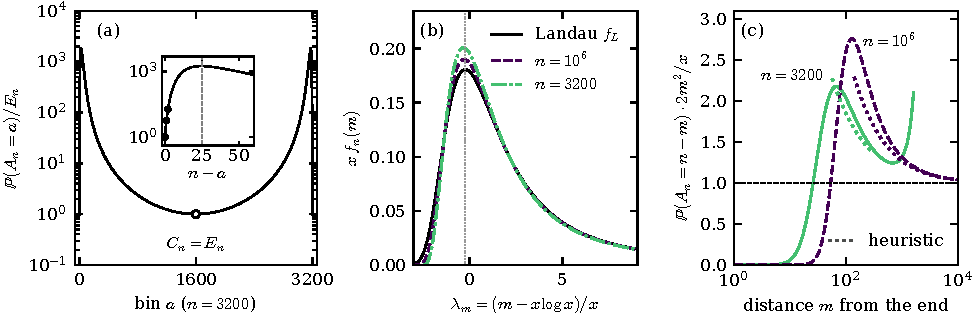
\includegraphics[width=\textwidth]{figures/shape}
\caption{The elephant walk at its crossing. (a) The law of $A_n$ at
$n=3200$ and its crossing $x=11.5468$, divided by the end $E_n$. The center
equals the end, and the law rises from each end to a mode and falls to the
center. The inset shows the last 60 bins, with dots at bins $n$, $n-1$ and
$n-2$. The end is below its neighbor, and the modes are 25 steps from each
end (dashed). (b) The law of $M_n$, scaled as $xf_n(m)$, against
$\lambda_m=(m-x\log x)/x$, with the Landau density $f_L$. The dotted line is
its mode $\lambda_0$. (c) The tail $\Prob(A_n=n-m)$ divided by $x/(2m^2)$.
The dashed line is the limit 1 of Theorem~\ref{thm:profile}. The rise of
the $n=3200$ curve near $m=n/2$ comes from the mirror term $f_n(n-m)$. The
dotted curves are the heuristic correction $1+x(2\log m+2\gamma-3)/m$, drawn
for $2x\log x\le m\le n/x$. At $n=10^6$ we use $x=22.4407$, the root $g_n$.
The second-order formula of Theorem~\ref{thm:erw-crossing}(b) puts the
crossing at $22.4399$.}
\label{fig:shape}
\end{figure}

\subsection{The bulk and the tail}

Let $\CP_n$ be the law of $\sum_{d=1}^{n-1}dN_d$, where the $N_d$ are
independent Poisson variables with means $x/(d(d+1))$. Its generating
function is $\exp\{x\sum_{d<n}(s^d-1)/(d(d+1))\}$, and for $n=\infty$ it is
$\exp\{x\chi(s)\}$ with $\chi(s)=(1-s)\log(1-s)/s$. Most minority steps come
from flipped families that do not overlap. By Lemma~\ref{lem:subtree} the
expected number of flipped vertices whose subtree has size $d$ is exactly
$x/(d(d+1))$, so the total size of the flipped families is close to a
compound Poisson sum. Two flips in the same family are rare when
$x^2\log n/n$ is small.

\begin{theorem}[compound Poisson bulk]\label{thm:cp}
For $n\ge2$ and $0<\varepsilon\le\frac14$,
\[
 \sup_{m\ge0}\bigl\lvert f_n(m)-\CP_n(m)\bigr\rvert\le\delta_B
 :=\frac{x^2\log n}{n}+\frac{4x^2}{n}e^{4x^2/n}+\frac{4x^2(H_n^2+H_n)}{n}.
\]
\end{theorem}

The proof is in Appendix~\ref{app:shape}. For $x^2\le n$ the bound is
$O(x^2\log^2n/n)$. It is additive, so at the crossing it says nothing for
$n\le10^6$ ($\delta_B$ is about $0.46$ at $n=10^6$). Numerically $\CP_n$ is
much closer to $f_n$ than this bound says. At $n=10^6$ and $x=22.4407$ the
largest value of $\lvert f_n(m)/\CP_n(m)-1\rvert$ over $1\le m\le10^4$ is
$3.5\cdot10^{-4}$. Near $m=n/2$ the relative error is larger. At $n=1600$
and $3200$ the ratio $f_n/\CP_n$ falls to $0.931$ and $0.956$ at $m=n/2$.

Let $f_L$ be the Landau density, defined by
$\int_{\mathbb R}e^{-u\lambda}f_L(\lambda)\,d\lambda=u^u$ for $u>0$. Its mode
is $\lambda_0=-0.2227829813$. We put $\lambda_m=(m-x\log x)/x$. The Landau
law appears because families of size $d$ are flipped at rate about $x/d^2$.
The families of size up to about $x$ add up to nearly their mean $x\log x$,
and the few families of size of order $x$ give fluctuations of order $x$.
So the bulk of $M_n$ sits near $x\log x$ and has width of order $x$.

\begin{theorem}[Landau limit]\label{thm:landau}
Let $n\ge2$ and $x\ge1$.
\begin{enumerate}[(a)]
\item For all integers $m\ge0$,
\[
 \bigl\lvert x\,\CP_n(m)-f_L(\lambda_m)\bigr\rvert\le E_L
 :=e^{2x/n}\Bigl[\frac{99.7\log x+517}{x}+\frac{4x}{n}\Bigr]+\frac2{\pi^2}e^{-\pi^2x/2}.
\]
\item If also $\varepsilon\le\frac14$, then
$\sup_m\lvert xf_n(m)-f_L(\lambda_m)\rvert\le E_L+x\delta_B$. So
$(M_n-x\log x)/x$ converges in law to the Landau law when $x\to\infty$ and
$x^3\log^2n/n\to0$, in particular at the crossing.
\item Let $\varepsilon\le\frac14$, and let $\kappa_L>0$ satisfy
$f_L(\lambda_0)-f_L(\lambda)\ge\kappa_L\min\{1,(\lambda-\lambda_0)^2\}$ for
all real $\lambda$. Put
$E'=E_L+x\delta_B+16x^2H_n/n^2+\lVert f_L''\rVert_\infty/(8x^2)$. If
$E'<\kappa_L/2$ and $m_h\le n/4$, then every mode $m$ of $f_n$ satisfies
$\lvert m-x\log x-\lambda_0x\rvert\le x\sqrt{2E'/\kappa_L}$, and so does
every $m^*$.
\end{enumerate}
\end{theorem}

The proof is in Appendix~\ref{app:shape}. A constant $\kappa_L$ as in (c)
exists if $f_L''(\lambda_0)<0$. Indeed, Taylor's theorem then gives
$c,\delta>0$ with $f_L(\lambda_0)-f_L(\lambda)\ge c(\lambda-\lambda_0)^2$ for
$\lvert\lambda-\lambda_0\rvert\le\delta$. The Landau law is stable, so $f_L$
is unimodal~\cite{yamazato1978}, and the difference is at least $c\delta^2$
for $\lvert\lambda-\lambda_0\rvert\ge\delta$. So $\kappa_L=c\min\{1,\delta^2\}$
works. We computed $f_L''(\lambda_0)=-0.0789$ by quadrature with 25 digits,
but we did not certify its sign, so the existence of $\kappa_L$ rests on
this computation. Given $\kappa_L$, part (c) gives
$m^*=x\log x-0.2228x+O(\sqrt{x\log x})$ at the crossing for all large $n$,
but not effectively.

The best constant is numerically
$\kappa_L\approx0.0262$, and then $E'<\kappa_L/2$ needs
$x\gtrsim1.3\cdot10^5$, that is, $\log n\gtrsim6.5\cdot10^4$ at the
crossing. So at the sizes we can compute the evidence for the mode is
numerical. At every tested crossing $m^*$ equals the mode of $\CP_n$. It is
$m^*=21,25,29,33,38$ at $n=1600,3200,6400,12800,25600$, and $m^*=47$ and
$64$ at $n=10^5$ and $10^6$ with $x=g_n$ in place of $x_n$. A heuristic
expansion one order further, which we have not proved, gives
$x\log x-0.222783x-0.535021\log x+0.549151+o(1)$ for the mode of
$\CP_\infty$. At $x=10\cdot2^k$ for $0\le k\le10$ it differs from the
computed mode, interpolated between integers, by at most $0.28$. The
difference is largest at $x=10$ and shrinks as $x$ grows.

\begin{theorem}[the tail]\label{thm:profile}
Let $x=n\varepsilon\ge1$ depend on $n$ with $x\log^2n/n\to0$, and let
$\omega_n\to\infty$ with $\omega_nx\log^2(x+1)=o(n)$. There is $\eta_n\to0$,
depending only on $n$, $x$ and $\omega_n$, such that for all large $n$ and
all $m$ with $\omega_nx\log^2(x+1)\le m\le n/2$,
\[
 \frac x2(1-\eta_n)\Bigl[\frac1{m(m+1)}+\frac1{(n-m)(n-m+1)}\Bigr]
 \le\Prob(A_n=n-m)\le\frac{x(1+\eta_n)}{2m(m+1)}+\frac12f_n(\lceil n/2\rceil),
\]
and $f_n(\lceil n/2\rceil)\le\frac{4x}{n^2}(1+\eta_n)$. In particular
$\Prob(A_n=n-m)=\frac{x}{2m^2}(1+o(1))$ uniformly for
$\omega_nx\log^2(x+1)\le m\le\delta'_nn$, for any $\delta'_n\to0$. For
$m=un$ with $u\in[u_0,\frac12]$ and $u_0>0$ fixed,
\[
 \frac{x}{2n^2}\bigl(u^{-2}+(1-u)^{-2}\bigr)(1-o(1))\le\Prob(A_n=n-m)
 \le\frac{x}{2n^2}\bigl(u^{-2}+4\bigr)(1+o(1)).
\]
\end{theorem}

The proof is in Appendix~\ref{app:shape}, from
Theorems~\ref{thm:B-local-lower}, \ref{thm:B-cum-upper}
and~\ref{thm:B-local-upper}. The constant is $\frac12$ because, for
$m\ll n$, bin $n-m$ is reached through a family of size $m$ only when
$X_1=+1$. For example, at $n=10^6$, $x=22.4407$ and $m=10^4$ the exact ratio
$\Prob(A_n=n-m)/(x/m^2)$ is $0.51889$. The explicit bounds behind the
theorem are weak at the sizes we can compute. At the crossing, the lower
bound of Theorem~\ref{thm:B-local-lower} says something only for
$164\le m\le400$ at $n=1600$ and for $118\le m\le2215$ at $n=3200$. The
upper bound of Theorem~\ref{thm:B-local-upper} is useful at the center and
the crossing only from $n\approx1.1\cdot10^8$, where its factor is about
$1.75$. The tail is not proved for $m$ between $x\log x$ and $x\log^2x$, and
for $m$ of order $n$ the upper bound on the mirror term $f_n(n-m)$ holds
only up to a constant. Heuristically, $\CP_n$ suggests
$f_n(m)\,m(m+1)/x\approx1+x(2\log m+2\gamma-3)/m$ at moderate $m$. This
factor is still about $2$ near $m=70$ when $n=1600$, so there the tail looks
like $x/m^2$ and not $x/(2m^2)$.

\begin{remark}[the center value]\label{rem:center-value}
For the center alone, Theorem~\ref{thm:erw-bounds}(c) is sharper. It gives
$C_n=\frac{4\varepsilon}{n+2}\,n^{2\varepsilon}e^{O(\varepsilon)}$, with
explicit constants, whenever $\varepsilon(1+\log n)\le\frac1{100}$.
Corollary~\ref{cor:B-center} gives only
$C_n=\frac{4x}{n^2}\bigl(1+O(\sqrt{x\log^2n/n})\bigr)$, and this is the form
that the proof of Theorem~\ref{thm:shape} uses.
\end{remark}

\subsection{The shape at the crossing}

\begin{theorem}[shape at the crossing]\label{thm:shape}
Let $n$ be even and let $x\in[2,n^{1/4}]$ satisfy $C_n=E_n$. There are
absolute constants $C_{\rm w}$ and $n_0$ such that the following hold for
$n\ge n_0$.
\begin{enumerate}[(a)]
\item $\Prob(A_n=n-1)>E_n$.
\item $\Prob(A_n=a)>C_n$ for every $1\le a\le n-1$ with
$\lvert a-h\rvert\ge C_{\rm w}n^{3/4}(x\log^2n)^{1/4}$.
\item If $E'<\kappa_L/2$ for a constant $\kappa_L$ as in
Theorem~\ref{thm:landau}(c), then $m^*$ satisfies the bound of
Theorem~\ref{thm:landau}(c).
\end{enumerate}
\end{theorem}

Part (a) is Theorem~\ref{thm:dip}, since $x\ge2>2(1-\varepsilon)$. Part (c)
is Theorem~\ref{thm:landau}(c), since $m_h=O(x\log^2x)\le n/4$ for large $n$
by Lemma~\ref{lem:B-mode}. Part (b) is proved in Appendix~\ref{app:shape}.
By Theorem~\ref{thm:erw-crossing} the crossing $x_n$ lies in $[2,n^{1/4}]$
for all large $n$. We did not compute $C_{\rm w}$ or $n_0$, and $n_0$ is at least
of order $10^8$ because the proof uses Corollary~\ref{cor:B-center}. The
window has this size because, at distance $t$ from $h$, the main term of
the law exceeds its value at $h$ by a factor of about $1+12t^2/n^2$, while
Corollary~\ref{cor:B-center} gives $C_n$ only up to a relative error of
order $(x\log^2n/n)^{1/2}$. Inside the window the proof gives nothing, and
closing it needs second differences of the law.

\begin{conjecture}[convexity between the humps]\label{conj:convex}
For every $n\ge10$, at $x=x_n$, the second difference
$\Prob(A_n=a-1)-2\Prob(A_n=a)+\Prob(A_n=a+1)$ is strictly positive for
$2m^*+1\le a\le n-2m^*-1$.
\end{conjecture}

With the symmetry of the law, the conjecture makes the law strictly convex
on $[2m^*,n-2m^*]$, so $h$ is its unique minimizer there (the 2 central bins
for odd $n$). For large even $n$ the other bins are covered by
Theorem~\ref{thm:shape}(b), since $m^*=O(x\log^2x)$. Indeed, at the
distance $\ell_0$ of Lemma~\ref{lem:B-mode}, which is $O(x\log x)$, the law
is at least $x/(4\ell_0(\ell_0+1))$ by Theorem~\ref{thm:B-local-lower} and
Lemma~\ref{lem:B-mode}, and by Theorem~\ref{thm:profile} it is smaller than
this at every distance $m\ge\omega_nx\log^2(x+1)$, for any $\omega_n$ that
tends to infinity slowly enough. So the conjecture and
Theorem~\ref{thm:shape} together would show that the center is the unique
interior minimum for all large even $n$.

The conjecture holds for every $10\le n\le600$ and for
$n=1600,3200,6400,12800,25600$. We predicted the cases $100\le n\le600$ and
$n=6400,12800,25600$ before computing them, and we checked $10\le n\le99$
and $n=1600,3200$ afterwards. The version on the closed range
$[2m^*,n-2m^*]$ is false for $n=10$, $11$, $17$ to $22$, $30$ to $35$ and
$48$ to $51$, and in each of these cases only the 2 endpoints fail. It holds
for every checked $n\ge52$. Along $n=1600,3200,6400,12800,25600$ the second
difference is positive on $[a_1,n-a_1]$ with $a_1=33,39,45,51,57$, while
$2m^*=42,50,58,66,76$. So the margin $2m^*-a_1=9,11,13,15,19$ grows with
$n$.

We can only explain the convexity heuristically. In our computations $f_n$
itself is not convex on $[2m^*,n-2m^*]$. It has a concave stretch where
$n-m$ lies between $m_h+1$ and about $0.68(xn^2)^{1/3}$. In the full law
this stretch is added to the tail $x/(2r^2)$ of the other branch,
with $r=n-a$, whose second difference $3x/r^4$ beats the concave curvature
of order $x^2/(n^2r^3)$. So the convexity is a cancellation between the 2
branches.

At every crossing where we computed the whole law, the law of $A_n$ has 2
humps. It rises from each end to a mode at distance $m^*$ and falls from
there to the center (to the 2 equal central bins for odd $n$). So for even
$n$ its first difference changes sign exactly 3 times. We observed this for
every $10\le n\le600$ and on the grid $n=50\cdot2^k\le25600$.
Figure~\ref{fig:shape} shows it at $n=3200$.
